
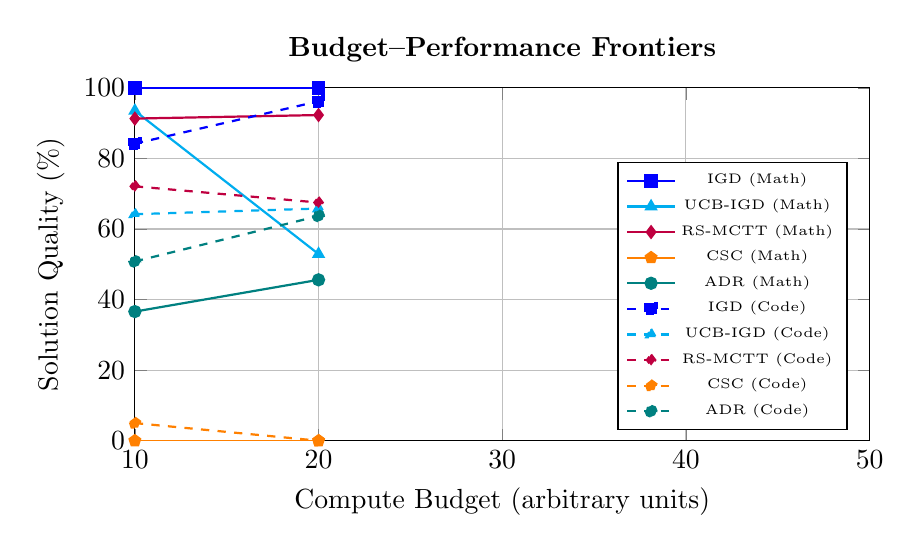
\begin{tikzpicture}
\begin{axis}[
    title={\textbf{Budget--Performance Frontiers}},
    xlabel={Compute Budget (arbitrary units)},
    ylabel={Solution Quality (\%)},
    xmin=10, xmax=50,
    ymin=0, ymax=100,
    xtick={10, 20, 30, 40, 50},
    ytick={0, 20, 40, 60, 80, 100},
    legend pos=south east,
    grid=major,
    width=0.9\textwidth,
    height=0.5\textwidth,
    legend style={font=\tiny},
]

\addplot[color=blue,mark=square*, thick] coordinates {
    (10, 100.0)
    (20, 100.0)
};
\addlegendentry{IGD (Math)}

\addplot[color=cyan,mark=triangle*, thick] coordinates {
    (10, 93.5)
    (20, 52.9)
};
\addlegendentry{UCB-IGD (Math)}

\addplot[color=purple,mark=diamond*, thick] coordinates {
    (10, 91.3)
    (20, 92.3)
};
\addlegendentry{RS-MCTT (Math)}

\addplot[color=orange,mark=pentagon*, thick] coordinates {
    (10, 0.0)
    (20, 0.0)
};
\addlegendentry{CSC (Math)}

\addplot[color=teal,mark=otimes*, thick] coordinates {
    (10, 36.6)
    (20, 45.6)
};
\addlegendentry{ADR (Math)}

\addplot[color=blue,mark=square*, dashed, thick] coordinates {
    (10, 84.2)
    (20, 96.2)
};
\addlegendentry{IGD (Code)}

\addplot[color=cyan,mark=triangle*, dashed, thick] coordinates {
    (10, 64.2)
    (20, 65.8)
};
\addlegendentry{UCB-IGD (Code)}

\addplot[color=purple,mark=diamond*, dashed, thick] coordinates {
    (10, 72.1)
    (20, 67.5)
};
\addlegendentry{RS-MCTT (Code)}

\addplot[color=orange,mark=pentagon*, dashed, thick] coordinates {
    (10, 5.0)
    (20, 0.0)
};
\addlegendentry{CSC (Code)}

\addplot[color=teal,mark=otimes*, dashed, thick] coordinates {
    (10, 50.8)
    (20, 63.7)
};
\addlegendentry{ADR (Code)}

\end{axis}
\end{tikzpicture}
